% $Id: nsf_description.tex 3089 2012-10-23 21:38:10Z nkraft $


\part{Computing Research Infrastructure Concept}
A \textit{Systematic Literature Review (SLR)} is a rigorous, standardized process by which researchers identify and analyze published evidence to draw broad conclusions about a phenomenon or research question.
The systematic, comprehensive, and reproducible nature of SLRs leads to findings that are less prone to bias and omissions than are s typical of the traditional \textit{ad hoc} literature review.
Given the frequency of empirical studies in software engineering (SE), the domain is well-suited for SLRs.
Although SLRs are increasingly recognized as vital to the SE discipline, the lack of infrastructure to support this effort-intensive, largely manual process results in barriers that inhibit their widespread adoption.
Building upon the results of our CI-P grant (NSF-1305395), the primary goal of this CI-NEW project is to build infrastructure to reduce these barriers and increase adoption of SLRs in SE.
For the sake of this proposal, we define \textit{infrastructure} to include both the back-end data storage and interchange, as well as the front-end user tools that support specific SLR steps.
Our target community comprises SE researchers who already conduct SLRs, SE researchers who will be more likely to conduct SLRs if the barriers are removed, SLR tool builders, and industry consumers of SE research results. 
The primary objectives of this CI-NEW project are to: 
\begin{itemize*}
	\vspace{-6pt}
	\item Build an extensive SLR support infrastructure;
	\item Ensure the infrastructure is flexible enough to incorporate existing and new tools; and
	\item Validate the usefulness of the infrastructure with members of the target community.
\end{itemize*}
\vspace*{-4pt }


\section{Introduction}
\label{sec:intro}

%\newcommand{\SHAW}{{\em {\sffamily BRIDGE}}}
 In their recent   2018 IEEE Software paper ``Bridging the Gap
From Research to Practical Advice'', 
Le~Goues, Shaw et al.~\cite{Goues18}
  lamented the poor connection between research discoveries and practitioner needs. To bridge that
 gap, they proposed  ``a system that allows researchers and
practitioners to reliably synthesize research results into actionable, real-world guidance,'' and literature reviews that make ``explicit recommendations on practice,
clearly labeled with strength of recommendation reflecting the level of rigor of the underlying evidence.''
There is a clear need for such a system: 
\bi
\item
On average, SE research   papers  earn less than one citation per paper~\cite{Mathew_2018}.
\item
This means that researchers and practitioners may miss important information.  
\item
Something needs to be done to stop so much research being not cited, forgotten, and hence wasted. 
\ei
Systematic Literature Reviews (SLRs) are one of the key approaches researchers use to systematically identify, analyze, and synthesize the research on a particular topic~\cite{Kitchenham:04,Kitchenham_Charters:07,Kitchenham-etal:04}.
The goal of an SLR is to provide a general overview of the current state of knowledge regarding topics or questions of interest.
Therefore, SLRs could be a key method to address the goals of 
Le  Goues,  Shaw  et  al.
Based on our own experience in the SLR and more general literature review space~\cite{Yu2018,Yu2019,Mathew_2018,mathewSoft18,Menzies89,hassler2014outcomes,%
carver2013identifying,%
hassler2016identification,%
carver13z,%
Kakar_Carver_2012,%
Carver-etal:13,%
Al-Zubidy-Carver:14},
we have a thorough understanding of many of the technical challenges proposed by Le  Goues,  Shaw  et  al.

One of the primary limitations of the current SLR approach is that it is a heavily manual and time consuming work requiring weeks to months of effort.
For example, 
a recent study reports taking over 400 hours to complete the ``selection process'' (which is only one of the parts required to complete  an SLR)~\cite{Hassler:14}. 
%This same study reports taking 4 man-hours to review the quality of results that took seconds of computer time using an automated technique.
Hence, while the concept of an SLR is quite applicable to the Le  Goues,  Shaw  et  al. challenge, in its current state it may {\em not} be suitable (since it is so slow).

\begin{table}
\caption{A sample of the manual and automatic {\em methods} available for exploring the SE literature.
The point of this proposal is to offer the infrastructure 
that lets  SE
community decide   how to make best use of these methods.
Note that this list is incomplete since researchers are
regularly proposing new approaches. Note also that while we present this list as a {\em linear} process (running from top to bottom), 
SLRs are usually a {\em cyclic process} where analysts make multiple iterations  across  these methods.}\label{tbl:overview}
\begin{center}
 {\small
  \begin{tabular}{p{1.5cm}|p{5.5cm}|p{8.3cm}}
    \rowcolor{gray}   & \textcolor{white}{Primarily manual methods} & \textcolor{white}{Automated AI-based text mining methods }  \\
    \hline
    1a. 
    \newline Define \newline research \newline question &   Read many papers (a very slow process)~\cite{kitchenham2004evidence,keele2007guidelines,marshall2013tools}. If there was a repository on prior questions we could explore them. &
    \bii
    \item {\em Dcluster:} Clustering documents with (e.g.) topic modeling~\cite{Mathew_2018};
    \item {\em Qcluster:} Cluster old queries to find common patterns in queries (and results);
    \item Find the gaps (clusters with low frequencies).
    \eii  \\\hline\rowcolor{blue!10}
    1b. \newline Identify  keywords& Extract keywords from research question topics and known related literature &
    \bii
    \item Extract candidate words from {\em Qclusters};
    \item Use feature selection (e.g. TF-IDF or RELIEF on support vectors);
    \item Auditing the keywords with synonym discovery (PCA~\cite{Wold1987Principal}, Word2Vec~\cite{mikolov2013efficient}). 
    \item Use of information extraction tools~\cite{Cruzes2007Automated}. 
    \eii \\
    \hline
    1c.\newline Create search string  & 
    \bii
    \item
    Use synonyms of keywords to identify terms for search string.
    \item
    Using subject matter experts (hard, they are hard to find).
    \item
    Use of gold standard to refine the search string~\cite{zhang2011empirical}.
    \eii &
    \bii
    \item Construct most informative search strings using  active learning~\cite{Yu2018,Yu2019};
    \item Using  SVMs, cull terms  explore those found most often
    far from hyperspace boundary;
    \item Apply Word2Vec~\cite{mikolov2013efficient} to extend query with keyword synonyms (as done in \cite{georgeLN}).
    \eii \\
    \hline\rowcolor{blue!10}
    2. \newline Search databases \cite{kitchenham2004evidence,keele2007guidelines}& \bii
    \item
    Snowballing~\cite{jalali2012systematic}.
    \item
    Use various permutations of search string in each database (sometimes requiring multiple searches per database) 
    \eii & AI
    not required for this task. However, with automatic tool supports, the time required for this task can be  greatly reduced. 
    \\
    \hline
    3. \newline Select \newline relevant papers&Current practice: a mostly manual process~\cite{kitchenham2004evidence,keele2007guidelines,hassler2016identification}&
    \bii
    \item Use active learning trained/updated on human review results to recommend what next to be reviewed~\cite{Yu2018,Yu2019}.
    \item Try initializing queries with results from {\em Qcluster}~\cite{Pan2010A}. 
    \item Explore using information other than title and abstracts, e.g. use full-text information or summary of text~\cite{summary1,summary2,summary3} 
    \eii\\
    \hline\rowcolor{blue!10}
    4. \newline Assess\newline quality  & Some checklists (number of subjects, type of studies, e.g bad smells)~\cite{kitchenham2004evidence,keele2007guidelines} & Not currently explored
    by AI tools~\cite{marshall2013tools}. This might be a matter of entity recognition~\cite{manning-EtAl:2014:P14-5} over checklist but really cannot be definitive at this time. %This is an area where we hope some share data and shared conventions on how to integrate tools would enable more experiment and more tools in the future. 
    \\    \hline
    5. \newline Extract data & Manual process: reading the the actual papers. E.g. run over a pdf and add mark ups over the text (so you can localize where you look)~\cite{kitchenham2004evidence,keele2007guidelines}.  & Topic modeling and visualization tools might help here~\cite{Felizardo2010An,Torres2012Automatic}\\
    \hline\rowcolor{blue!10}
    6. \newline Synthesis of results &  Manual work with help using  tools~\cite{kitchenham2004evidence,keele2007guidelines,marshall2013tools}. & Visualization might be able to help this process~\cite{Cruzes2007Using,Felizardo2011Analysing,Felizardo2010An} \\
    \hline
    7. \newline Summary of papers&   & Not done right now. But summarizing of technical artifacts is an emerging natural language technology~\cite{gambhir2017recent} so we can look to much improvement in this area, in the near future. \\\hline
  \end{tabular}
 
}
\end{center}


\end{table} 

In order to make the SLR approach more amenable to addressing the Le  Goues,  Shaw  et  al. challenge, we posit that the latest generation of AI text mining methods can be used to greatly reduce the required effort while improving the quality of the outcomes. For a sample of those text mining methods, see \tbl{overview}.


The range of methods in \tbl{overview} is very broad and  is growing all the time. 
How can the SE community cope with this growing number of  new and highly experimental methods?
More importantly, how can the SE community evolve an consensus of what is a ``valid'' use of the \tbl{overview} methods (where ``valid'' means that researcher1 will accept the conclusions made by researcher2 using some subset of \tbl{overview}). 
Such a consensus is absolutely essential  to provide scientific repeatability, improve coverage, reduce human labor and errors, and allow for iteration and improvement of SE knowledge. 


This rest of this proposal
discusses an infrastructure that includes all the methods from \tbl{overview} that 
 addresses the Le  Goues,  Shaw  et  al. challenge.  
 That infrastructure, which we call {\IT} (the SLR Artificial Intelligence Toolkit), will include a ``glue'' system where tools can be easily interconnected. Graduate students funded under this work would then become text mining consultants helping the international community conduct their literature searches using our tools. As a result of this work we would (a)~assist many researchers to better
 explore the literature and (b)~learn what parts of \tbl{overview} are most/least useful.
 
We have strong reasons to believe that  {\IT}
will be a very efficient tool. 
Recent work
shows that 
the SE corpus of research papers is not particularly large. 
Mathew, Menzies et al.~\cite{Mathew_2018,mathewSoft18}
found 35,391  published papers in the period 1992-2016
at major SE venues (conferences and journals).
Of course, they could have studied many more papers from many more venues. However, Mathew, Menzies et al. also found that the  clusters within these documents were stable despite
numerous {\em ablations} (removing  pairs of venues, picked at random,
then recreating the clusters). That is, they found no benefit in explore more than $\approx10^4$ papers. 
This observation  has  two practical implications:
\bi
\item
While $10^4$  papers is too many   for humans to read,  this is a relatively small corpus for natural processing; i.e.  it is 
practical to suggest applying
AI text mining methods to the SE literature.
\item
Since that space is not so large,
  it should be possible to pre-compute and cache certain queries, thus reducing the time required to process future queries, as  proposed in \tbl{overview} (see last column of the row ``1a. Define research question'').
\ei

\vspace{6pt}
\section{Infrastructure Description}
~\\
\noindent
{\bf {\em Fundamental infrastructure}} (what is to be developed):
\bi
\item
To address the Le  Goues,  Shaw  et  al. challenge we  propose   an integrated environment called {\IT} that is a
 mash-up of manual SLR tools
and the AI-based tools.

Currently, we plan to add all the methods of \tbl{overview} to {\IT}. Other methods might be added later, as time permits.


The premise of {\IT} is that AI is useful,  {\bf but only if it is augmented
with human-in-the-loop expertise}.
{\IT} will  identify methods
appropriate for using combinations of human and AI tools to read  large numbers of SE research reports.  

{\IT}  will help researchers produce unbiased, repeatable, comprehensive SLRs. Lastly, {\IT} will be the ``playground'' within which the SE community might evolve
a consensus on what methods to use/avoid in the creation of ``valid'' results.
\ei
\ei 
 
\noindent
{\bf {\em  Tools, resources, and data sets}} (describe ancillary resources to be developed and integrated into the infrastructure system)
\bi
\item
 {\IT} will include all the methods of \tbl{overview}
 plus a lightweight ``glue''
 notation for combining the inputs
 of one method to the outputs of another (this ``glue''
 is discussed further in \tion{combine}). Sample
 {\IT} scripts will show how  to run our tools.
 {\IT} will also include  sample data sets (comprising data taken from SE papers) that researchers can use for:
\be
\item Tutorial materials to   learn our tools;
\item  Materials with baseline results that researchers can use to test
new AI-boosted SLR methods against prior data sets.
\item Data  from older literature reviews that can  
  ``jump-start'' new literature reviews.
\ee


%\item
%Figure~\ref{figure-ResearchEnabled} shows the {\IT} conceptual model.
\ei
 {\bf {\em  User services}}  (services   integrated into the infrastructure 
(including mechanisms by which researchers will gain access to the infrastructure):
\bi
\item 
{\IT} will be a set of open source tools, hosted in a public Github repository for free use by industrial and research practitioners. 
\item
Graduate students funded under this grant will 
(a)~provide systems support for researchers performing literature reviews using {\IT};
(b)~create plug-ins for missing functionality. 
\item
{\IT}  will provide a lightweight API and data interchange facilities so users can build workflows by plugging-in existing tools.
{\IT}  will use
AI to (partially) automate   search and selection of materials; extraction, evaluation, and synthesis of those papers; and updates of published
SLRs.


\ei 
{\bf {\em  Community engagement}} (how the community will be engaged in the design, development, and management of the infrastructure):
\bi
\item
Our goal with {\IT} is 100+ SLRs conducted using these tools. We do not plan to conduct all these 100+ SLRs ourselves.  Rather,    {\IT}
is a community infrastructure project that will support many researchers conducting better 
literature reviews. 
To create that community infrastructure, we will:
\be
\item As described above: we will release {\IT} as an open-source toolkit; assign graduate student time to systems support for other research teams using these tools.
\item
Also, as described in our research plan (\S\ref{sec:Plan}), we will  run numerous  training sessions where the PI, co-PI, or graduate students working on this grant will work one-on-one with interested
researchers to assist them in using {\IT}. While these sessions will
partial be tutorial in nature, we will also use these sessions
to do participant observation of users applying our tools (so we can learn what parts of our tools are especially useful/useless).
\item Further, we will convene regular meetings of a
review panel  where international researchers will assess our toolkits and make recommendations for change. To open up these review
panel meetings to the general research population, we will run workshops on  advanced SLR-based technology. While some sessions of those meetings will be devoted to {\IT}, we will also run other sessions where researchers can present any other approach to enhance SLRs.
\ee
\ei
{\bf {\em Community outreach:}}  (plans for ongoing outreach to develop a diverse user community):
\bi
\item
Successful implementation of {\IT} will serve three communities shown in 
Figure~\ref{figure-ResearchEnabled} :
\be

\begin{figure}[!t]
	\centering
	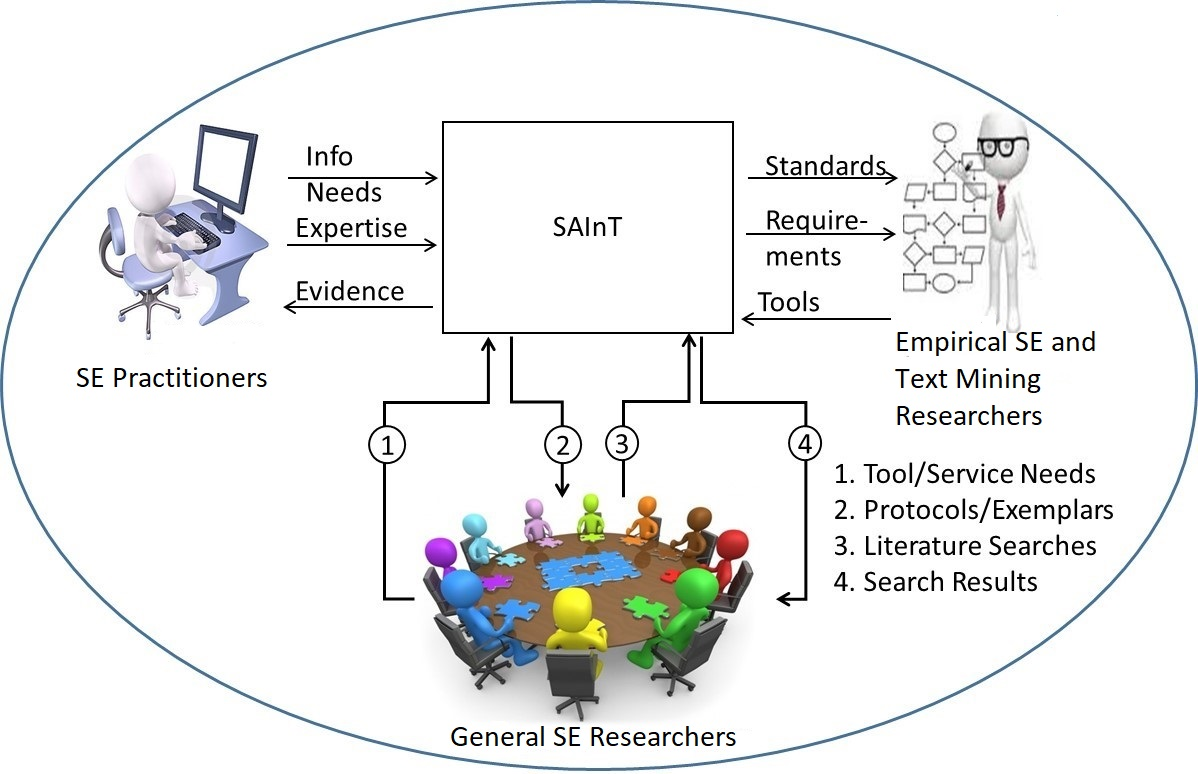
\includegraphics[width=4.5in]{ResearchEnabled}
	\caption{Communities Serviced by {\IT}.}
	\label{figure-ResearchEnabled}
\end{figure}
\item {\em Community \#1: General Software Engineering Researchers}
 

 One reason to augment standard SLRs with AI tools (as done in {\IT}) is that the SE field urgently  needs to rethink its core premises using more of the current evidence.
We say this since currently there is much
disagreement on what many factors most effect software projects.
For example, according to Passos et al.,  developers often assume that the lessons they learn from a few past projects are general to all their future projects. 
They comment, ``past experiences were taken into account without much consideration for their context''~\cite{Pa11}. 
 J{\o}rgensen \& Gruschke offer a similar warning. 
They report that the supposed software engineering ``gurus'' rarely use lessons from past projects to improve their future reasoning and that such poor past advice can be detrimental to new projects~\cite{Jo09}.
 Other studies have shown some widely-held views are now questionable given new evidence.
	Devanbu et al. examined responses from 564 Microsoft software developers from around
	the world. 
	They comment programmer beliefs can vary with each project, but do not necessarily correspond with actual evidence in that project~\cite{De16}. 

The Le~Goues, Shaw et al.~\cite{Goues18} paper  characterizes such uncertainties
as symptoms of a researcher
  community that is poorly defining its research outputs. They say:
  \begin{quote}
  {\em When engineers seek answers to their practical problems, ``perfect'' scientific knowledge is not always available. If it's not, engineers readily accept ``good-enough'' evidence: case studies, small-scale experiments, blog posts, or even advice from acknowledged experts.}~\cite{Goues18} 
  \end{quote}
Their challenge to the community is to provide better ``good-enough'' evidence. In this proposal,
we explore the application of AI tools to text mining to provide such good enough evidence via AI-augmented literature reviews.
\item
{\em Community \#2:  Empirical Software Engineering and Text Mining Researchers}
We also plan to support these researchers by providing a platform to experiment  with  different techniques  and  workflows. Empirical software engineering researchers have established some recommended workflows (e.g. pilot search and keyword refinement~\cite{keele2007guidelines}) and strategies (e.g. snowballing~\cite{jalali2012systematic}) to improve the efficiency and quality of SLRs. Meanwhile, many text mining researchers have selected SLRs as case studies to test the effectiveness of different machine learning algorithms (e.g. active learning~\cite{Yu2018} and visual text mining~\cite{Felizardo2010An}). {\IT} as a platform will facilitate the testing of mix-and-matching different workflows, strategies, and algorithms, thus benefit the research of both empirical software engineering and text mining. In addition, {\IT} will be beneficial as a testbed for latest developed algorithms from text mining and machine learning, e.g. word2vec, deep neural networks, named entity recognition, part-of-speech tagging, etc.

\item {\em Community \#3: Software Engineering Practitioners}
In addition to the benefits to researchers described above, the numerous consumers that utilize the results of SLRs will also benefit from the work.  
Practitioners and executives in industry utilize SLR results to identify best practices and to guide decision making.  
Industrial software engineers will benefit from more applied and relevant research that they can commission.
Other researchers have already begun building methods (e.g. Visual Abstracts~\cite{VisualAbstracts}) for representing the findings of SLRs in a format that is useful to practitioners.
By helping researchers produce more SLRs that represent all of the literature, {\IT} will help the results presented to industry be more complete and accurate.
\ee
\ei
\vspace{8pt}

\section{Systematic Literature Review Process}
\label{sec:process}
To help ensure the rigor required to conduct an unbiased, repeatable, and thoroughly documented SLR, the researchers perform three phases.
At each phase of the process, multiple researchers work independently and then meet to resolve any differences through discussion~\cite{Kitchenham:04, Kitchenham_Charters:07, Biolchini-etal:05}.
First, to provide transparency, in the \textit{planning} phase, the researchers develop a formal protocol that explicitly defines a plan for:
\vspace{-8pt}
\begin{enumerate}
	\item A comprehensive literature \textbf{search} to identify candidate primary studies of interest, including an explicit description of the research questions, the databases to be searched, and the search string to be used.
	\vspace{-4pt}
	\item A culling of the candidate studies to \textbf{select} those that are relevant, including detailed inclusion and exclusion criteria to make the selection more objective.
	\vspace{-4pt}
	\item A \textbf{quality assessment} of each selected study using a predefined quality assessment rubric.
	\vspace{-4pt}
	\item \textbf{Data extraction} from each selected study using a data extraction form to ensure consistency across all included studies.
	\vspace{-4pt}
	\item A \textbf{synthesis} of the extracted data to answer the research question(s).
\end{enumerate}
\vspace{-4pt}
Second, in the \textit{execution} phase, researchers perform each of the steps in the defined protocol.
Finally, in the \textit{documentation} phase, researchers explicitly document the exact process followed and the findings from the synthesis.  

While research reports typically describe the SLR process as being sequential, our interactions with SLR researchers reveal it to be much more iterative~\cite{Carver-etal:13, Hassler-etal:14}.
As shown in Figure~\ref{figure-SLR-Process}, the results of one step may require re-planning of later steps or even re-planning and re-execution of previous steps.
Feedback from SLR researchers suggests that an ongoing monitoring process helps to ensure that the research team is in agreement and that the SLR is proceeding according to a valid, documented plan.
Each step is preceded by a form of stage-gate that serves as a quality checkpoint.
Therefore, prior to each step, the SLR team reviews and revises the plan as needed.
This monitoring allows the SLR team to maintain confidence in the results. 

Because SLR teams are often distributed, there is a need for appropriate communication facilities.  
The SLR team often must interchange large data sets -- including full articles at early phases.
In addition to the resources required to perform the individual SLR steps, resources must be expended on management and coordination of the team.
Thus, the production of a single SLR is a difficult and resource intensive effort.

As a result of the formal planning and systematic process described above, the SLR approach is fundamentally different from the \textit{ad hoc} approach in that SLRs:
\vspace{-8pt}
\begin{itemize} 
	\item Reduce the potential of accidentally omitting important papers;
	\vspace{-8pt}
	\item Are more likely to be executed by a team of researchers working collectively;
	\vspace{-8pt}
	\item Are more likely to provide independent, stand-alone value as a research result; and
	\vspace{-8pt}
	\item Are more likely to be replicated and updated by other researchers.
\end{itemize}
\vspace{-4pt}


\part{Preliminary Work}
% $Id: part_prelim.tex 3073 2012-10-23 17:55:38Z jcarver $

We have performed initial work to gather community needs and identify necessary characteristics and features for the infrastructure. Section~\ref{sec:prelim:needs} describes the community needs we have identified through our own experiences and our interactions with the community. Section~\ref{sec:prelim:tools} describes our current view of the infrastructure required to address the identified community needs.

% vim:syntax=tex


%\section{Proposed Requirements}
\section{Identification of Community Needs}
\label{sec:prelim:needs}
% $Id: sec_prelim_needs.tex 3089 2012-10-23 21:38:10Z nkraft $

As a starting point for planning the infrastructure, we have identified a set of important community needs, which will be iterated upon during the course of the project. The important community needs we identified include, improved support for:
\vspace*{-4pt}
\begin{enumerate*}
	\item{Coordination among multiple (possibly distributed) researchers}
	\item{Protocol review by the community}
	\item{Interaction with different literature databases}
	\begin{enumerate*}
		\item{Federated search}
		\item{Search string manipulation and translation}
		\item{Duplicate result elimination}
		\item{External citation management tool interoperation}
	\end{enumerate*}
	\item{Quality assessment}
	\item{Data extraction}
\end{enumerate*}
\vspace*{-4pt}

Section~\ref{sub:sources} describes the three data sources used to gather these needs. Section~\ref{sub:analysis} provides a detailed analysis of the data sources to illustrate the origing of these community needs.

\subsection{Overview of Data Sources}
\label{sub:sources}

To gather community needs, we used three data sources: a graduate course by PI Carver (Section~\ref{sub:SLR:course}), a review of published SLRs (Section~\ref{sub:SLR:review}), and a survey of SLR authors (Section~\ref{sub:SLR:survey}).

\subsubsection{PI Carver's SLR Course}
\label{sub:SLR:course}

In Spring 2012, PI Carver taught a graduate ``Advanced Empirical Software Engineering'' course. There were eight PhD students enrolled in the course (four Computer Science PhD students and four Management Information Systems PhD students). The main focus of this course was for the students to learn about and conduct SLRs. As such, the course had two primary goals:
\vspace*{-4pt}
\begin{enumerate*}
	\item Each student conducted an SLR as a semester-long  project. Realizing that most SLRs cannot be completed within one semester, it was expected that work would continue beyond the semester to make these SLRs publishable. At this point, two of these papers have been accepted in conferences~\cite{Thompson_et_al_2012,Kakar_Carver_2012}, at least five other papers will be submitted to various journals in the near future, including \emph{European Journal of Information Systems} and \emph{Information and Software Technology}, and most of them will become part of the students' dissertations.
	\item Second, throughout the semester, class time was devoted to discussing each student's SLR and to evaluating the SLR process. Each student wrote a report at the end of the semester describing their SLR process, noting where they had difficulties, and suggesting improvements to the SLR process.
\end{enumerate*}
\vspace*{-4pt}

In addition, each student acted as a second reader for the SLR of one of their classmates. PI Carver oversaw all SLRs, provided input on the protocols and helped to resolve any conflicts during the paper selection/data extraction process. Due to the effort required to conduct these reviews, it was not possible for every paper to be reviewed by two reviewers. So, at each elimination stage of the SLR process (i.e. title elimination, abstract elimination and full paper elimination), the second reader reviewed a random subset of 10-20\% of the excluded papers to ensure that the primary author was not prematurely excluding papers that could be relevant. When the primary author reached the data extraction stage, the second reader reviewed the full data extraction for a subset of the papers.

In addition to the interaction among the primary author and the second reader throughout the semester, a large portion of the class meeting time was devoted to discussing each SLR. Each student had the opportunity to present his protocol and received feedback from his classmates. The class also spent a substantial amount of time discussing the logistics of the SLR process and identifying common problems encountered by multiple students. By the end of the course each student produced two deliverables:
\vspace*{-4pt}
\begin{enumerate*}
\item An initial version of the SLR, which in most cases needed further revision to become publication-ready; and
\item A report describing his experiences with following the standard SLR process, including specific areas in which he encountered difficulties. It is these reports that provided the bulk of the information described Section~\ref{sub:analysis}.
\end{enumerate*}
\vspace*{-4pt}

\subsubsection{SLR Literature Review}
\label{sub:SLR:review}

For the second source of data, we performed a thorough literature search and identified 214 published SLRs. We analyzed those SLR papers to identify strengths and weaknesses in the current SLR process, including areas in which tool support could be helpful. During the review of these papers, we used the following data extraction process:
\vspace*{-4pt}
\begin{enumerate*}
\item Determine whether the SLR protocol was explicitly described
\item Review the description of the protocol to:
\vspace*{-4pt}
   \begin{enumerate*}
	\item Note databases used and the search strategy for those databases
	\item Note any deviations from Kitchenham's process (whether stated explicitly or not)
	\item Note any tools used
	\item Note any difficulties described about the process
   \end{enumerate*}
\vspace*{-4pt}
\item Look for a ``lessons learned'' section to get more details
\item Note anything else particularly interesting about the SLR process in the paper
\end{enumerate*}
\vspace*{-4pt}
The information extracted from this analysis is included in Section~\ref{sub:analysis},
and the list of 214 published SLRs is included among the cited references at the end of this proposal.

\subsubsection{Survey of SLR Authors}
\label{sub:SLR:survey}

Finally, to obtain more detailed insight into the SLR process, we developed a list of SLR authors from the list of published SLRs identified in Section~\ref{sub:SLR:review}. We sent a survey to all of those authors that asked them to detail: the SLR process followed, where they had difficulties in the SLR process, where they spent their time during the SLR process, and which aspects of the SLR process were most in need of tool support. The results of the 50+ survey responses are included in the discussion in Section~\ref{sub:analysis}.

\subsection{Analysis of SLR Process}
\label{sub:analysis}

This section uses data gathered from the three data sources described in Section~\ref{sub:sources} to analyze the steps in the SLR process. The goal of the analysis is to identify aspects of the SLR process that SLR authors found particularly difficult, highlighting community needs for tool support of the SLR process. This section is organized around the major phases of the SLR process: Section~\ref{sub:proto:plan} discusses general issues regarding Protocol Planning and Section~\ref{sub:proto:items} focuses on specific protocol items. For the sake of continuity, we discuss data from all three data sources together under each heading. As we discuss each phase of the SLR process, we specify the identified community needs.


\subsubsection{Protocol Planning}
\label{sub:proto:plan}

This section describes general information pertaining to protocol development. Information about detailed protocol items appears in Section~\ref{sub:proto:items}. During PI Carver's course, the students' stated that the frequent discussion of their protocols with each other and with PI Carver helped in the development and refinement of the protocols. The students also found it helpful for their SLR process to be guided by PI Carver, who is experienced in conducting SLRs. These experiences are not unique to PI Carver's course. Our review of the SLR literature suggests that many SLRs are performed by students as part of their thesis work. Guidance from a more experienced researcher/reviewer is crucial to the accuracy and success of the review~\cite{EMendes_2005}. The community needs identified in this phase are:
\vspace*{-4pt}
\begin{itemize*}
\begin{bfseries}
\item Protocols may have to be revised and edited during the SLR process
\item Protocols need to be socialized among peers for review and feedback
\item Novice researchers need the ability to interact with a more experienced research during the planning and execution of the SLR
\end{bfseries}
\end{itemize*}
\vspace*{-4pt}

\subsubsection{Protocol Items}
\label{sub:proto:items}

This subsection describes the results obtained for protocol items P2-P6.

\paragraph{P2. Research Questions}

The research question(s) are arguably the most important aspect of the protocol because they drive the remainder of the protocol. Based on the experiences in PI Carver's course, it is clear that the research question(s) have to be appropriately scoped. If they are too broad, they will generate too many papers to reasonably evaluate in one SLR. Conversely, if they are too narrow, they will not generate enough papers to draw useful conclusions. Scoping of the research question(s) is an activity in which feedback from more experienced researchers could be quite beneficial. The community need identified in this section is:
\vspace*{-4pt}
\begin{itemize*}
\begin{bfseries}
\item Research question(s) must be properly scoped
\item Expert feedback is beneficial to formulating appropriate research question(s)
\end{bfseries}
\end{itemize*}
\vspace*{-4pt}

\paragraph{P3. Search Strategy}

The search strategy includes database selection and creation of one or more search string(s) from the research question(s). Creating the search string(s) can be an iterative process as the researcher attempts to define the appropriate set of keywords and synonyms that cover the research space. This section first discusses issues with the databases and then issues with the search strings.

Regarding databases, SLR researchers typically search multiple databases, which may have different functionality. Based on the experiences in PI Carver's course, we can make the following observations regarding the databases. First, databases have different behavior regarding the search strings. For example, in some cases changing the order of the keywords changes the result set. In other cases, Boolean logic does not work as expected. As a result, researchers must develop a different set of search strings for each database. Second, the advanced search functionality differs across databases. In some cases, the advanced search interface returns different results than the basic search interface, even if the same search string is used. Third, there is a large overlap in the literature covered by the databases commonly used for SLRs, creating the need to identify and remove duplicate studies from the result set. Fourth, databases differ in the content and format of the citation information provided. Finally, the databases are not consistent in their behavior regarding bulk export of references to a citation manager.

Similar problems with the peculiarities of the databases were also reported by the papers in our literature review (e.g., \cite{LChen_et_al_2009,EladioDomınguez_et_al_2012,MuhammadSarmadAli_et_al_2010,LianpingChen_et_al_2011,SoniaMontagud_et_al_2012,MehwishRiaz_et_al_2009,IvoneiFreitasdaSilva_et_al_2011,EMendes_2005}). A relatively small number of researchers used EndNote to facilitate the removal of duplicate papers (e.g., \cite{LianpingChen_et_al_2011}) while most performed the task manually.

Regarding the search strings in general (i.e. not including differences among databases), the experiences in PI Carver's course resulted in the following observations. First, adding a '*' at the end of a key term helps to identify variant spellings. Second, when using a common term like ``Open Source,'' restrict the search to the title, abstract and keywords to limit the number of irrelevant hits. Third, in some cases a large number of relevant papers were not returned by the initial search, causing the search string to be refined based upon the results of a secondary search, i.e. reviewing references in the identified papers.

This information suggests the following community needs:
\vspace*{-4pt}

\begin{itemize*}
\begin{bfseries}
\item The ability to search multiple databases in one tool
\item Automatic (or semi-automatic) manipulation of search string to accommodate peculiarities of various databases
\item Automatic elimination of duplicate results
\item The ability to export all citations in a common format (i.e. BibTex or EndNote)
\end{bfseries}
\end{itemize*}
\vspace*{-4pt}

\paragraph{P4. Identification of Primary Studies}

Once the search results are identified, the next step is to determine which papers should be included in the SLR. There are two aspects to this process: the definition of the inclusion/exclusion criteria and the process of actually determining which papers belong in the review. The SLR author survey indicated that selecting appropriate papers was the third most difficult and second most time consuming aspect of the SLR process. It was also the aspect second most in need of tool support.

PI Carver's course resulted in the following observations about the inclusion/exclusion criteria: 1) there is a need to ensure that it conforms to the goals of the current review rather than just being reused from other SLRs; 2) there is a need for expert review; 3) it should be as specific as possible; and 4) it may have to be reviewed and edited during the search process. 

PI Carver's course also resulted in the following observations about the paper selection process: 1) review of the titles and abstracts may not be sufficient for eliminating papers; 2) there is a need for a citation manager to keep track of the references; 3) have to manually examine or write a script to handle duplicate results across databases; 4) when searching for specific terms or content that may not be evident in the title/abstract/keywords, the addition of a quick scan of the full text of the paper may be useful for quickly eliminating irrelevant papers; 5) this step was very time consuming, especially having multiple reviews of papers; and 6) it is difficult to coordinate meeting times. 

The literature review showed that other authors reported the same or similar problems. For example, some researchers noted the difficulty of duplicate removal~\cite{DIKSjoeberg_et_al_2005}. Researchers used various tools for managing the papers: a ``citation manager,''~\cite{MuhammadSarmadAli_et_al_2010} or EndNote~\cite{SusanMMitchell_et_al_2009,LianpingChen_et_al_2011,HongyuPeiBreivold_et_al_2010}.

\vspace*{-4pt}
This information suggests the following community needs:
\begin{itemize*}
\begin{bfseries}
\item There is a need for expert review of inclusion/exclusion criteria
\item The citations need to be managed within the tool
\item The tool needs to interoperate with external citation management tools (e.g., BibTeX, EndNote)
\item There is a need to automate the elimination of duplicate papers
\item There is a need for management of the review process among the SLR team
\end{bfseries}
\end{itemize*}
\vspace*{-4pt}


\paragraph{P5. Quality Assessment}

Once a set of candidate primary studies has been identified, the next step is to perform a quality assessment to determine whether any should be excluded due to the unreliability of their results. The results of the SLR author survey showed that quality assessment was the second most difficult and third most time consuming aspect of the SLR process.

The experiences from PI Carver's course resulted in the following observations. First, the quality assessment checklist should be part of the data extraction form. Second, the quality criteria must be relevant to the specific topic and not just reused from a prior SLR. Third, the researcher must ensure that the quality assessment criteria will actually differentiate between papers of different quality. Finally, the quality assessment should be performed by at least two researchers to avoid bias. These observations suggest the following community needs:

\vspace*{-4pt}
\begin{itemize*}
\begin{bfseries}
\item There is a need for a mechanism to build appropriate quality assessment criteria
\item There is a need to facilitate multiple authors performing quality assessments independently
\end{bfseries}
\end{itemize*}
\vspace*{-4pt}

\paragraph{P6. Data Extraction}


Once the authors have arrived at a final set of papers that are to be included in the SLR, the next step data extraction. The results of the SLR author survey showed that extracting data from papers was the most difficult and most time consuming aspect of the SLR process. It was also the aspect that was the third most in need of tool support.

The experiences in PI Carver's course resulted in the following observations about the data extraction process. First, the data extraction form needs to be reviewed by an expert in SLRs and an expert in the domain of the review. Second, realize that the form may need to be refined throughout the process as the authors better understand the papers. Third, the extracted information needs to be reviewed by collaborators to eliminate any bias. Finally, there is a need for a tool that allows the extracted data to be easily recorded and analyzed across multiple papers. In our literature review, most researchers did not report the use of a tool for data extraction. We did find a few researchers using EndNote (e.g., \cite{CarlaPacheco_et_al_2012,LEfrizoni_et_al_2010,HongyuPeiBreivold_et_al_2012}) or a spreadsheet (e.g., \cite{LianpingChen_et_al_2011,HongyuPeiBreivold_et_al_2012,ShaukatAli_et_al_2010,SamirehJalali_et_al_2010}) to manage the data extraction process. These observations suggest the following community needs:
\begin{itemize*}
\begin{bfseries}
\item There is a need to facilitate expert review of the data extraction form
\item There is a need to support multiple authors extracting and reviewing data
\item There is a need to ease the recording and analysis of the extracted data
\end{bfseries}
\end{itemize*}


\subsection{Existing SLR tools}
Section~\ref{sub:existing:tools} described three tools that support various aspects of the SLR process. While RevMan / Archie does include desirable features, it is primarily designed for documenting and maintaining individual medical studies under the auspices of the Cochrane Collaboration. StaRt and SLuRp have a similar focus to our proposed infrastructure. This section briefly analyzes the StArt and SLuRp tools with regards to their match to the identified community needs.

StArt enforces a rigid interpretation of the SLR process. It requires the user to enter elements of the protocol, which are later used to mandate additional inputs before the user may proceed with conducting the review. While true to the original definition of the SLR protocol, this tool lacks the ability to support the iterative nature of the SLR process. As a result, evolution of the protocol during review process is cumbersome. In addition, StArt is designed to be a desktop application that supports a single user, thus, neglecting the collaborative nature of the SLR process.

SLuRp is web-based and allows multiple researchers to collaborate on the same SLR. However, it does not aid in the development of the search string.  While it does record the researchers' ratings about primary study selection and quality assessment, it does not support the resolution of disagreements among researchers. SLuRp does record bibliographic data for studies imported into the tool, but removal of duplicates and merging of conflicting entries is still a manual process. Finally, SLuRP lacks facilities to export bibliographic and other extracted data into commonly accepted formats for importation into specialized tools, such as EndNote or statistical packages.

Some other observations about these two tools highlight the need for the creation of a new infrastructure. Both follow a strict interpretation of the SLR process and do not fully support the inclusion, and use, of techniques such as snowballing to recover relevant studies that may have been missed due to the nature of database searches. StaRt does allow these techniques to be used during the piloting phase, but they cannot be included as a formal part of the review. Additionally, neither tool facilitates ongoing maintenance of reviews or the ability for researchers to build upon previous work. Prior search results, quality assessments and extracted data are not readily available for use in the updating of existing reviews or the construction of new reviews. 

% vim:syntax=tex


%\section{Proposed Solution}
\section{Infrastructure Characteristics and Features}
\label{sec:prelim:tools}
% $Id: sec_prelim_tools.tex 3078 2012-10-23 19:15:47Z nkraft $

While we realize that the activities of this planning grant, specifically those defined in Section~\ref{sec:needs}, may provide additional inputs that could change the community needs identified in Section~\ref{sec:prelim:needs}, we do not anticipate any significant changes in the focus of the project. As a result, to illustrate the proposed infrastructure, this section provides an overview of our proposed solution. We plan to develop a web-based cyberinfrastructure that will enable: 1) coordination among multiple (possibly distributed) researchers, 2) community review of protocols, 3) automated interaction with different databases, 4) improved quality assessment, and 5) simple, repeatable data extraction. 

\subsection{Addressing Community Needs}
Our approach to addressing each of these needs is described in the remainder of this section.

\paragraph{Coordination among multiple authors} The web-based nature of the infrastructure will enable researchers who are not collocated to collaborate on execution of the same SLR protocol. The description of each of the requirements below also highlight features that enable multiple authors to collaborate on the same SLR using the proposed infrastructure. 

\paragraph{Community review of protocols}
The first and arguably most important step of the SLR process is the development, documentation, and validation of the protocol. The protocol includes: the motivation for the study, the research question(s), the sources for the primary studies, the search strings, the inclusion and exclusion criteria, the data extraction information, and the process details for each step of the execution phase. During construction of the protocol, the tool will also allow for the collaboration and feedback among the members of the SLR team. Once completed, the infrastructure will provide a mechanism for the public review of the proposed protocol and allow for community feedback. This feature will help provide researchers with confidence that the protocol is sound and will increase the chances of publication, if it is well-executed.

\paragraph{Automated interaction with databases}
To support the time consuming process of searching for and identifying primary studies the tool will provide a number of features. First, it will support both manual and automated searching of multiple databases. Second, it will allow for manual importation or automated retrieval of search results. Third it will help researchers create robust search strings by analyzing the provided keywords and suggesting alternatives, based upon the history of previous SLRs. Fourth, the system will adapt the standardized search strings defined in the protocol to the idiosyncrasies of known databases, where possible. Fifth, the tool will automatically detect duplicate papers in the various result sets, perhaps by using DOIs. Upon completion of the search phase, the tool will allow multiple researchers to evaluate the search results against the predefined inclusion and exclusion criteria. As each researcher's evaluation is captured independently, the tool will also provide inter-rater agreement ratings and isolate studies in need of further discussion among the SLR team. 

\paragraph{Improved quality assessment}
Once the final set of candidate studies is determined, the tool will support the quality assessment for each study based on previously defined criteria. As different types of research (e.g., lab experiments, field studies, etc.) should be evaluated based on criteria appropriate for the design, the system will allow researchers to classify and subsequently evaluate, using the appropriate criteria, each of the identified primary studies. Again, using the history of previous SLRs, the tool will help the researcher refine the quality assessment criteria by suggesting additional criterion that are related to those specified by the researcher. Once again, as each researcher's evaluation is captured independently the tool will provide information regarding agreement among the researchers and facilitate resolution of any conflicts.

\paragraph{Simple, repeatable data extraction}
For the final set of studies, the tool will provide a mechanism to facilitate data extraction. For strictly quantitative data extraction, the tool will perform an automated comparison to determine agreement among the researchers. To evaluate the extraction of qualitative information, the tool will provide a facility for third-party evaluation of the researchers' data extractions. As with other portions of the system, a means of evaluating agreement among the researchers and resolving conflicts will be made available. As the SLR moves into the analysis and then documentation stages, the tool will permit researchers to export citation information, in various formats, and all data collected during the extraction phase. 

\subsection{Enabling Future Research}
As indicated in the previous section, as each SLR performed utilizing the tool is completed, all of its data will be made available for inclusion in subsequent reviews, with proper attribution to the original researchers. We envision that this feature will support the establishment of research communities focused on a given topic or domain. As new research is completed, studies can be added to the existing knowledge base and processed for inclusion in updated SLRs.

While the infrastructure initially targets the research community, inclusion of practitioners in the target community could provide additional possibilities. Practitioners may provide expert opinions and evaluations of SLR topics, or provide guidance related to important research questions that need to be answered. Furthermore, the system may facilitate the transfer of knowledge gained from research to practitioners in the field.

% vim:syntax=tex



%\part{Proposed Work}
\part{Remaining Work}
%The previous part of this proposal has provided many details about the goals and requirements for the proposed infrastructure.
The sections in this part provide details about the design, evaluation, and dissemination of the infrastructure.

%\section{Evaluation of Proposed Requirements}
\section{Identification of Community Needs}
\label{sec:needs}
% $Id: sec_needs.tex 3080 2012-10-23 19:33:43Z jcarver $

\vspace*{-4.5pt}
This section describes our plan to identify the consensus needs of the community
by supplementing and improving the preliminary community needs described in Section~\ref{sec:prelim:needs}
and by validating and prioritizing the improved community needs.
Our plan comprises the following tasks:
\begin{itemize*}
\setlength\itemindent{-1.15em}
\vspace*{-4.5pt}
\item[] \textbf{Data Collection and Analysis}
   \begin{enumerate*}
   \setlength\itemindent{-1.4em}
   \vspace*{-3pt}
   \item[T1.] Extract additional process details from published SLRs
   \item[T2.] Code additional survey responses from SLR authors
   \item[T3.] Analyze the extracted process details and coded survey responses
   \end{enumerate*}
\vspace*{-3pt}
\item[] \textbf{Evolution of Identified Community Needs}
   \begin{enumerate*}
   \setlength\itemindent{-1.4em}
   \vspace*{-3pt}
   \item[T4.] Supplement the preliminary community needs based on the analysis results
   \item[T5.] Solicit community feedback on the supplemented needs
   \item[T6.] Improve the supplemented community needs based on the community feedback
   \end{enumerate*}
\vspace*{-3pt}
\item[] \textbf{Validation and Prioritization of Identified Community Needs}
   \begin{enumerate*}
   \setlength\itemindent{-1.4em}
   \vspace*{-3pt}
   \item[T7.] Validate the improved community needs  using community evaluation
   \item[T8.] Solicit community input on the prioritization of the validated community needs 
   \item[T9.] Prioritize the validated community needs based on the community input
   \end{enumerate*}
   \vspace*{-9pt}
\end{itemize*}

\vspace*{-6pt}
Tasks T5 and T7 involve workshop organization.
The following paragraphs describe the workshop agendas.
Before each workshop we will post an announcement to the SEWORLD mailing list and send invitations to SLR authors.
We will also contact survey respondents that have expressed interest in this project.
After each workshop we will document activities and outcomes, post them to the project Wiki, and announce their availability.

\paragraph{Data Collection and Analysis}
Tasks T1--T3 involve the improvement of our preliminary analysis of process details from the published SLRs and survey responses from the SLR authors.
Task~T1 is to improve our preliminary analysis of the 214 published SLRs described earlier.
We will extract additional process details from each of the published SLRs to permit a more complete
analysis of the SLR process, including the difficulties that authors face and the strategies that they use to ease those difficulties.
%Task T2 is to improve our preliminary analysis of the 50+ survey responses that we received from authors of published SLRs.
Task T2 is to improve our preliminary analysis of the 50+ responses to our SLR author survey.
We will code additional author responses from each of the survey responses to permit a more complete
analysis of SLR process data, %the difficulties faced and of the needs identified by the respondents.
including labor-intensive, automatable process phases. %or in need of tool support.
Task T3 is to analyze all collected data. %results of Tasks T1 and T2.

\paragraph{Evolution of Identified Community Needs}
Tasks T4--T6 involve the evolution of the preliminary community needs. % (Section~\ref{sec:prelim:needs}).
Task T4 is to supplement the preliminary community needs based on the results of Task T3.
We will both refine existing and formulate new community needs based on the analysis results.
Task T5 is to solicit community feedback on the supplemented community needs that result from Task T4.
We will organize a half-day workshop at the 2013 International Conference on Software Engineering (ICSE'13). %,
%to be held May 2013 in San Francisco, CA.
Because an award notification would arrive just before the conference (in May),
participation is likely to be limited to those already planning to attend ICSE'13.
Thus, we will contact colleagues directly to request their feedback. %via other channels such as email and the project Wiki.
Task T6 is to improve the supplemented community needs based on the community feedback from Task T5. %we receive. %workshop outcomes.
%We will integrate suggestions from workshop participants and other community members who provide feedback via email or the project Wiki.

\paragraph{Validation and Prioritization of Community Needs}
Tasks T7--T9 involve the validation and prioritization of the improved community needs that result from Task T6.
Task T7 is to validate the improved community needs with help from the community.
We will organize a workshop at the 2013 International Symposium on Empirical Software Engineering and Measurement (ESEM).
During the day-long workshop, participants will refine and validate the improved community needs via a series of evaluation activities.
Time permitting, we will solicit participant input on the prioritization of the validated community needs.
Task T8 is to solicit additional community input related to prioritization of community needs.
We will solicit this input via a survey. %of community members.
Task T9 is to prioritize the validated community needs based on the community input from Task T8.
%We will integrate the results of Task T8.


% vim:syntax=tex


%\section{Evaluation of Proposed Solution}
\section{Infrastructure Characteristics and Features}
\label{sec:tools}
At those workshops, participants reviewed a range of
SLR support tools.
They found that SLRs still suffer from a lack of complete tool support.
According to a mapping study~\cite{Marshall-Brereton:13}, 11 SLR-related tools are described in the SE literature. 
Most of these tools (7 of 11) target the selection of studies to include in the review~\cite{MS:11,MS:13,MS:14,MS:21,MS:22}, the extraction of data~\cite{MS:12,MS:18,MS:21}, or the synthesis of data~\cite{MS:12,MS:16,MS:17,MS:20}.
Three of the other tools~\cite{MS:15,MS:19,MS:23} target the entire SLR process.
The remaining tool~\cite{MS:24} targets the identification of candidate studies.
Unfortunately, most of the tools identified by the mapping study~\cite{Marshall-Brereton:13} are either in early stages of development or are not freely available.
Furthermore, only two of those tools~\cite{MS:18,MS:23} have been evaluated independently~\cite{Marshall-Brereton:13}.

Starting from the list in the mapping study~\cite{Marshall-Brereton:13}, we selected the three tools that were specifically focused on SLRs, targeted multiple phases of the SLR process, and were freely available (SLuRP, StART, and SLR-Tool).
We also identified two additional tools not covered in the mapping study (SLRTOOL and Parsifal).
(Note that we excluded ReVis and PEx from our evaluation because there are designed to support single phases of the SLR process. However, we will include those tools in our construction of SAInT, where appropriate.)
Using information from the literature and our own evaluation of the tools, we documented each tool's features and limitations~\cite{Al-Zubidy-Carver:14}.
Based on the detailed results of the Community Workshops, we analyzed each tool's features to determine whether they covered any or all of the desired features.
We iterated the results of our analysis with each tool's authors to ensure we had accurately characterized them.
Table~\ref{table-tools} summarizes our findings and shows that none of the tools fully support the requirements for the entire SLR process.

\begin{table}
	\centering
	\caption{Tools - \ding{51} = fully covered; \ding{119} = partially covered; \ding{109} = not covered. The important observation to be made from this table is that all the current SLR tools
	offer partial support for parts of the SLR process. This table lends suppport
	to the design premises of {\IT}; i.e. (a)~that
	no single tool offers support for the entirety of SLRs; and (b)~best results come from combining
	the capabilities of multiple tools.}
	\resizebox{\textwidth}{!}{
	\begin{tabular}{|m{1.8cm}|m{1.4cm}|m{1.5cm}|m{1.5cm}|m{1.4cm}|m{1.3cm}|m{1.5cm}|m{2cm}|m{1.5cm}|m{2.1cm}|}
%	\begin{tabular}{|p{1cm}|c|c|c|c|c|c|c|c|c|}		
\hline
~                               & Planning & Searching & Selection & Quality Assessment & Data Extraction & Data Synthesis & Presentation & Report Generation & Coordination \\ \hline
\rowcolor{blue!10} Connection to \tbl{overview} &Rows 1a,1b,1c&Row 2&Row 3&Row 4&Row 5&Row 6&\multicolumn{2}{c|}{Row 7}\\\hline
SLuRP                       & \centering\ding{119}        & \centering\ding{119}         & \centering\ding{119}         & \centering\ding{119}                  & \centering\ding{119}               & \centering\ding{119}              & \centering\ding{119}            & \centering\ding{119}                 & \ding{119}           \\ \hline
StArt                          & \centering\ding{119}        & \centering\ding{119}         & \centering\ding{119}         & \centering\ding{119}                  & \centering\ding{119}               & \centering\ding{119}              & \centering\ding{119}            & \centering\ding{119}                 & \ding{109}            \\ \hline
SLR-Tool                    & \centering\ding{119}        & \centering\ding{119}         & \centering\ding{119}         & \centering\ding{119}                  & \centering\ding{119}               & \centering\ding{119}              & \centering\ding{119}            & \centering\ding{119}                 & \ding{109}            \\ \hline
SLRTOOL 				& \centering\ding{119}         &
\centering\ding{109}         & \centering\ding{119}         & \centering\ding{119}                  & \centering\ding{119}               & \centering\ding{119}              & \centering\ding{119}            & \centering\ding{119}                 & \ding{119}            \\ \hline
Parsifal & 						\centering\ding{119}        & \centering\ding{119}         & \centering\ding{119}         & \centering\ding{119}                  & \centering\ding{119}               & \centering\ding{119}              & \centering\ding{119}            & \centering\ding{119}                 & \ding{119}           \\ \hline
\end{tabular}
}

%51 = F
%109 = N
%119 = P

	\label{table-tools}
\end{table}

The problem of incomplete SLR tool support is not restricted to just the SE community.
The medical community often uses the following tools to support SLRs.
Note that neither tool provides much support for the planning or execution phases of the SLR process:
\bi
\item
RevMan~\cite{RevMan} focuses primarily on the documentation phase of SLRs performed under the guidelines of the Cochrane Collaboration. 
It facilitates the preparation of formatted tables and version tracking. 
\item
Archie~\cite{Archie} is the central repository for RevMan and is used to store completed reviews. 
\ei
Review of the medical literature and interaction with an MD who participate in our first workshop showed that the medical community faces many of the same problems faced by the SE community.
Many of these barriers relate to the difficulties faced during searching~\cite{Bouamrane-etal:11, Frunza-etal:10, Young-Ward:01, Zwolsman-etal:13, Zwolsman-etal:12, Lai-etal:10}.
\vspace{8pt}

\newpage
\part{Project Plan}
% $Id: part_plan.tex 3065 2012-10-23 12:31:42Z nkraft $

In this part we describe the project management plan and project timeline.

% vim:syntax=tex


\section{Project Management}
\label{sec:mgmt}
Development of the SLR Infrastructure will be accomplished through an iterative program management structure shown in Figure~\ref{fig-plan}.  
Program management will ensure the coordination across the development of the feature sets. 
We will assign one of the PIs or Senior Personnel to serve as the dedicated project team lead for each feature set, where a feature set includes all functionality in one or more of the SLR phases.
Features that support planning, coordination, and monitoring will be shared among the team leads as a separate feature set.
We will also assign a graduate student to work closely with the team lead. 
In addition, we will hire professional developers from the Center for Advanced Public Safety (CAPS) (\url{http://www.caps.ua.edu}) at the University of Alabama, with which PI Carver is affiliated. 
CAPS engages in innovative, state-of-the-art software research and development.
CAPS has approximately 50 full-time developers that are highly skilled in various development platforms.
Most developers hold Master's degrees in computer science, with some pursuing PhDs.
CAPS has successfully deployed over 50 software products and systems as well as many web-based analytics portals and other website systems.
This expertise fits well with the development needs for SAInT.


Each project will use an agile approach. 
To help ensure appropriate \textit{quality of service}, our emphasis will be on developing maintainable code that is extendable and will minimize the operational costs to continue the operations of the SLR infrastructure once the grant period is completed.  
We will prominently consider sustainability principles during the design and construction of the infrastructure.
We have defined the scope of development so that it will generate a valuable set of infrastructure tools, yet be narrow enough to be completed and be sustainable beyond the grant period.

\begin{figure}
	\centering
	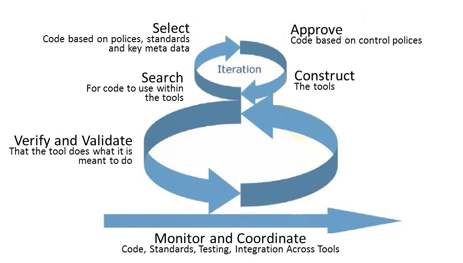
\includegraphics[width=5in]{Plan}
	\caption{High-Level Architecture}
	\label{fig-plan}
\end{figure}

Once at steady-state, each project will use 3-week (4 per quarter) sprints to develop and enhance their components. 
At the end of each sprint, integration across the feature sets will ensure coordination and compatibility.  
Experienced SLR authors and existing tool developers will have access to resulting sprint builds and have input into the product backlogs and priority assignments of these items (see attached support letters).  
Each team will construct a backlog of features that need to be developed for their specific feature set.
With the aid of the users of the specific features providing input, the project lead for each team will act as product owners to prioritize the backlog for each sprint.  
The graduate student will be responsible for high-level architecture and design decisions, including investigating various trade-offs in implementation choices.
The CAPS developers will implement and test the features in each sprint.
During the execution of the sprints and during the retrospectives at the end of the sprints we will identify cross-feature relationships and add them to the backlog for the appropriate feature sets.
The user communities for each of the feature sets will have the capability to be active testers to ensure features perform as expected.  

%The assignment of the feature sets will be based on needed expertise, current capabilities and programmatic learning objectives.  
%As an example of the programmatic learning objectives, CS students will be assigned to take the lead for core backplane tier features, while MIS students will take the lead for planning, coordination and monitoring features.  
%This assignment will draw on their experiences, coursework and career objectives.   
%Collectively the CS and MIS students will learn to work together and extend their professional comfort drawing upon the strengths of one another. 

\section{Project Schedule}
\label{sec:sched}
The schedule in Table~\ref{table-schedule} provides an overview of the number of development sprints planned for each quarter.  
It also provide an overview of other major activities planned each quarter such as Program Coordination and reviews by external (i.e., Non-UA) SLR  tool developers.  
Other reviews will be conducted at least every 9 months by external SLR authors and practitioners. 
The workshops for External Tool Developers and SLR Authors are also shown.   
The last item on the schedule shows the efforts that will take place to ensure the infrastructure is sustainable beyond the life of this grant. 

The project schedule considers multiple constraints and goals, for example:
\vspace{-8pt}
\begin{itemize}
	\item SAInT Feature Integration will ramp up during the first quarter (conducting 3 sprints) and then reach a steady state of 4 sprints for each of the next four quarters.  
	At the mid-point of the grant period, we will conduct a workshop with non-UA tool builders and SLR authors.  
	\item Preparing for the workshop and responding to feedback will reduce the number of sprints in the Winter 2017-18 quarter (after which 4 sprints per quarter will resume).  
	\item In the last 3 quarters of the project, the number of sprints will be ramped down as more user testing and training activities ramp up.
	\vspace{-4pt}
\end{itemize}
\vspace{-4pt}

\begin{table}
	\centering
	\caption{Project Schedule}
	\label{table-schedule}
	\begin{table}[!bth]
\caption{Project Schedule}
\label{tab:Schedule}
{\footnotesize 
\begin{tabular}{p{.48\textwidth}|c@{~}c@{~}c@{~}c|c@{~}c@{~}c@{~}c|c@{~}c@{~}c@{~}c|}
\cline{2-13}
	&   \multicolumn{12}{c|}{\textbf{Quarters}}  \\
	&   \multicolumn{4}{c}{Year 1}      & \multicolumn{4}{c}{Year 2}     & \multicolumn{4}{c|}{Year 3}      \\
	Tasks                          & Fall & Wint & Spr & Sum & Fall & Wint & Spr & Sum & Fall & Wint & Spr & Sum \\
\hline
	Program Coordination           & x    & x    & x   & x   & x    & x    & x   & x   & x    & x    & x   & x   \\
\hline
	\textbf{Initialize} - Analyze \& choose AI/Text-mining tools \& Identify data outputs for SLR phases       & x    & x    & x   & x   &     &     &    &    &     &     &    &    \\
\hline
	\textbf{Compose} - AI/Text-mining tools \& Data model for SLR phases       & x    & x    & x   & x   & x    &  x   & x   & x   & x    &  x   &x    & x  \\
\hline
	\textbf{Popularize} - Conduct one-on-one case studies  &     &     &    & x   &     &  x   &    & x   &     & x    &    & x   \\
\hline
	\textbf{Popularize} - Workshops                     &      &      &      &  x   &      &     &     &     &      &      &     &   x  \\
\hline
	\textbf{Support} - Use Helpdesk &      &      &      &     & x     & x    &x     & x    & x     & x     & x    & x    \\
\hline
	\textbf{Audit} - Tune AI/Text-mining approaches \& Conduct human-based studies                     &  x    &   x   &   x  &  x   &    x  &   x  &  x  &   x  &   x   &  x   &   x  & x   \\\cline{2-13}

\end{tabular}
}
\end{table}
\end{table}


\part{Results of Prior NSF Support}
% $Id: part_prior.tex 3082 2012-10-23 19:38:07Z jcarver $

NSF CCF-0915559 (PI: Kraft, Co-PI: Carver), (2009-present), Title: \emph{SHF: Small: Collaborative Research: Improved Code Clone Categorization}. In this project, PIs Kraft and Carver are developing and evaluating methods for categorizing code clone information to make it useful for developers. This project has supported the work of six graduate students. To date, this project has led to six workshop/conference~\cite{Beard_et_al:11,Carver_et_al:11,Chatterji_et_al:11,Chatterji_et_al:10,Chatterji_et_al:12,Corley-etal:12} papers and three journal publications~\cite{Lukins_et_al:10,JeremyRPate_et_al_2011,Biggers-etal:12}.

Co-PI Hale has no results in the previous 5 years.

% vim:syntax=tex


% vim:syntax=tex
